\documentclass[notitlepage]{report}
\usepackage{graphicx}
\usepackage{listings}
\usepackage{multicol}
\usepackage{float}
\usepackage[section]{placeins}

\makeatletter
\newcommand*{\toccontents}{\@starttoc{toc}}
\makeatother

\begin{document}

\title{CS124 Individual Project  - Down the Scurvy Dog  Write Up}
\author{Owen Garland - owg1@aber.ac.uk}
\date{}
\maketitle
\toccontents
%\tableofcontents

\section{How to run this software}
Download the .jar file, then either double click on it in Windows, or from the command line on any OS run. use the -text flag to use the command line version. 

\begin{lstlisting}
  java -jar PirateApp.jar 
  java -jar PirateApp.jar -text
\end{lstlisting}

\section{Analysis}
The problem that I was given was to create a simple hangman like game that involved a pirate walking a plank, rather than the traditional hangman. The specification for the project recommended that I use the Java  to create a text based version of the game and then use the  Swing library to create a GUI. I was also given an interface for the game model. 

I was also given a small dictionary of words that would have to be used in the game. These words would need to be read in from the filesystem and then be used as the hidden words for the user to attempt to guess. This made it clear that I needed to create a class that could handle loading in text files in the given format. 

After examining the interface it became clear that I would need to create a game model class that would implement the interface I was given. I would then create two views of the game model, one text based and one graphical. 


\subsection{Requirements}
The application must: 
\begin{enumerate}
  \item Implement the GameModel Interface provided
  \item Read from the piratewords.txt file provided
  \item Provide a graphical and text based interface
  \item Be pirate themed
  \item Have a JUnit tests written for it
  \item Be packaged in a JAR file
\end{enumerate}

\subsection{Runtime Environment}
The application will be written in the latest version of Java, and using the Swing library. There was no target OS defined so it is assumed that it should be able to run on multiple platforms. I will be developing it on Linux, and then testing on Windows and Linux. Sadly I don�t have a Apple device to test on, however a JAR file that runs on Windows and Linux should work well on Mac as well. 

\subsection{My Solution}
I will be using the Model View Controller design pattern, as this will allow me to break the problem down into more logical constituent parts. The most import part of this design pattern is the model, as that is what actually performs the functions of the program. Thanks to the interface that I have been given the model will actually be quite easy to create as the needed functions and parameters are already defined for me, I just need to implement them. 

The view and controller functions of this design are merged into one for this implementation as the two views that I have to create, the text and GUI versions, can easily control how the game interacts with the model; making it unnecessary to create a controlling class. This saves time and again simplifies the design. 

In summary I will have the GameModel which is programmed from the interface given, and two view/controllers, one for the GUI and one for the text version of the game. 


\begin{figure}[!htb]
  \centering
  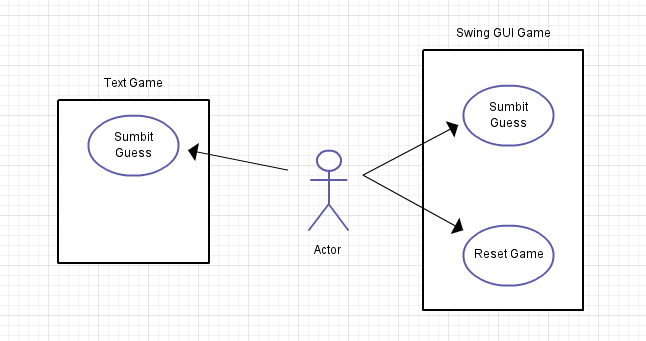
\includegraphics[scale=0.5]{UseCaseDiagram}
  \caption{This shows how the user will interact with the system}
  \label{fig:label}
\end{figure}

\section{Design}
I have already identified the need for a few classes in my analysis of the problem. Now I will go into more detail about what the classes will contain and how they will be organised. 

I have decided to only have five classes in my solution, one for running the main method and launching the application, one class for loading the piratewords.txt dictionary file, a game model class that will implement the interface that I was given, and then a text and gui class for the two different views of the games. 

\subsection{PirateApp}
This is the class that contains the Main method and runs the application. It handles a few small administration tasks such as reading in the command line arguments and creating an object of the Dictionary class for the game model to use. Then, depending on the command line options it will pass the model object across to either the SwingGame class or the Text Game class. 


\subsection{Dictionary}
This class will simply load a given text file from the filesystem, and parse it. It will also provide a method for randomly selecting a word from the loaded text file. In this case it will be set to load the piratewords.txt file that has been provided; however it was also used to load a text file with just one word in for the JUnit tests. 

\subsection{TextGame}
This class is actually a very small class, as it only really has one function, to take the users input from the command line, pass it to the GameModel and then display the results. It doesn�t even have any methods, I will just run a While loop in the constructor that takes the input until either the game is won or lost. 

\subsection{GameModel}
This is the most important class in the design as it performs all of the algorithms that the game uses. It implements the GameModelInterface that we were given in the specification. As well as the methods included in the interface I have also added a couple of methods that I thought would be useful. 

Firstly I have added a won() method, when called it will return true or false depending on if the user has won the game. This makes it easier for the view classes to know when the game has been finished. 

One extra feature that I decided to add was the ability to reset the game in the GUI version so the player could play again once they have won or lost the game (Or they give up on the word!). This required a new word to be selected from the Dictionary, so the selectNewWord() class will get a new random word.

\subsection{SwingGame}
This class is rather large in terms of code, that is because it will contain all of the data for how the GUI is to be presented and laid out. All of this code is contained within the createGui() method, this is just to keep it neat. The other methods are for the creation of popups or actions to be performed when a button is clicked. I have also created an AddButton() method that uses Callable to make the creation of a button and event listener/handler much easier. 

\begin{figure}
\subsection{Class Diagram} 
  \centerline{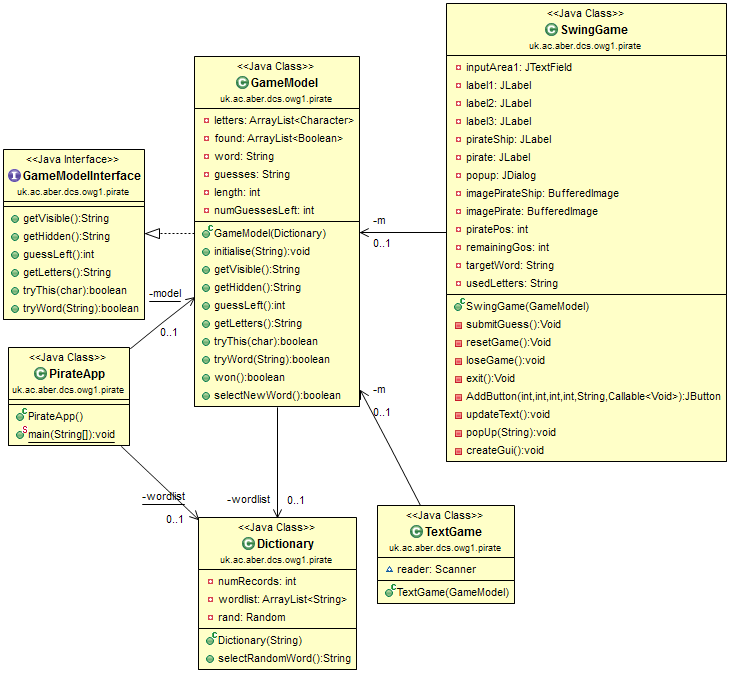
\includegraphics[scale=0.7]{ClassDiagram}}
  \caption{This shows how the different classes will be laid out}
  \label{fig:label}
\end{figure}

\begin{figure}
\subsection{Sequence Diagram}
  \centerline{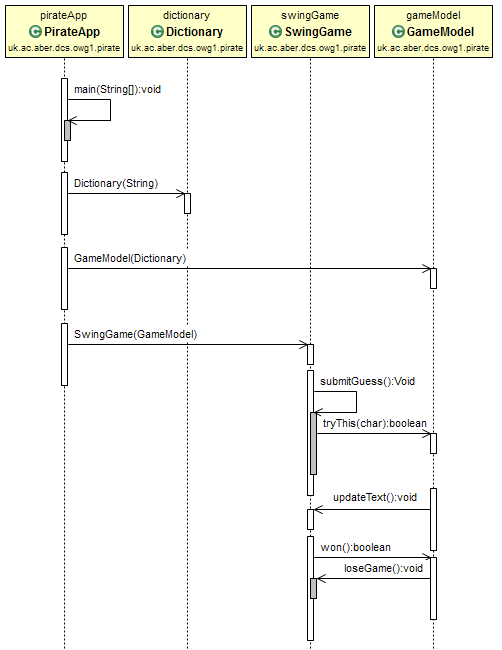
\includegraphics[scale=0.7]{SequenceDiagram}}
  \caption{This sequence Diagram shows what would happen if a user opened the application and submitted a character until they lost}
  \label{fig:label}
\end{figure}

\newpage

\section{Algorithm Design}
I believe that the easiest way of creating the actual hangman operation of the game, a hidden word that gets revealed, will be to have two arraylists, one character array that contains the letters in the hidden word, and then a boolean array that determines whether or not the character in the word has been found. So for example, I would have two arrays, that would be worked on to produce the visible data for the user. 

\begin{figure}[!htb]
  \centering
  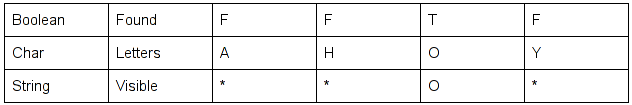
\includegraphics[scale=0.5]{table}
  \caption{This demonstrates how I will hide the word}
  \label{fig:label}
\end{figure}

The main algorithms for this application are all contained within the GameModel class, this is programmed from the GameModelInterafce, so it is clear what algorithms will be needed. Below is some pseudo code that explains how the main algorithms will work.

\subsection{Initialise}
This is a method in GameModel that will set up the needed ArrayLists for the game, based on the word that was passed to it. 

\begin{lstlisting}
for each character in word 
    letters.add(character)
    if(character == ' ')
	found.add(true)
    else
	found.add(false)

length = letters.size
\end{lstlisting}

\subsection{Get Visible}
This method will perform the operation that is demonstrated in figure 3. It simply performs an TRUE operation on the letters arraylist using the found arraylist. 

\begin{lstlisting}
for length
    if letter = ' '
	result += " "
    else if(found == true)
	result += letter
    else
	result += "*"

return result
\end{lstlisting}
 

\subsection{Try This}
This method takes a char as an argument called letter, and then tests whether the char is used in the word, and then if it is correct it sets the position that it is at in teh found array list to true, else it removes a guess from the number of guesses the player has. 

\begin{lstlisting}
correct = false;

for length
    ifletters.get(i) == letter
    found.set(i, true);
    correct = true;

if NOT correct AND letter not in guesses
    numGuessesLeft--
    guesses += letter + " "
else
    correct = true;

return correct;
\end{lstlisting}

\subsection{Try Word}
This method takes a String as an argument called guess. It simply test whether the guess is equal to the hidden word. If it is then it fill the found arraylist to true, if it isn�t correct however it removes five guesses from the remaining guesses left. 

\begin{lstlisting}
if guess == word
    found.fill = true
    return true
else    
    numGuessesLeft += -5
    return false
\end{lstlisting}

\subsection{Won}
This method isn't specified in the interface for GameModel but I think that it will make it easier to determine when the game has been won, rather than trying to calculate it in the view/controller areas. It just checks whether all of the elements in the found arraylist are true or not. If they are then the game has been won, if not then the game has not been won yet. This method returns a boolean value, true for won, false for not won.

\begin{lstlisting}
for each value in found
if value != true
    return false

return true
\end{lstlisting}

\section{Testing}
Here I shall test all of the inputs for my program, both from the command line and GUI. All of these tests are used with a test word file called word.txt. This file contains the two words "ahoy" and "ye"; this is done so that I know what the word to guess is.

\newpage
\begin{figure}
\subsection{Test results table}
  \centerline{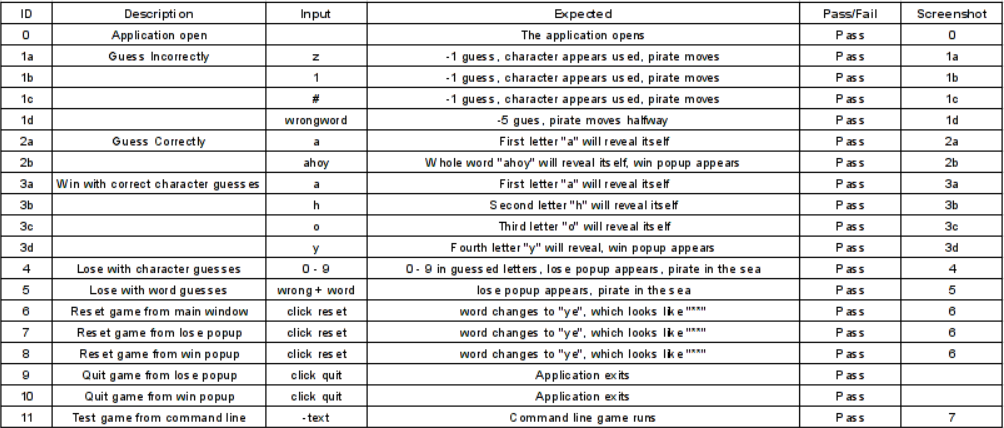
\includegraphics[scale=0.5]{testtable}}
  \label{fig:label}
\end{figure}


\newpage
\subsection{Test screenshots}
Screenshots of the application running. 
\begin{multicols}{2}

\begin{figure}[H]
\centering
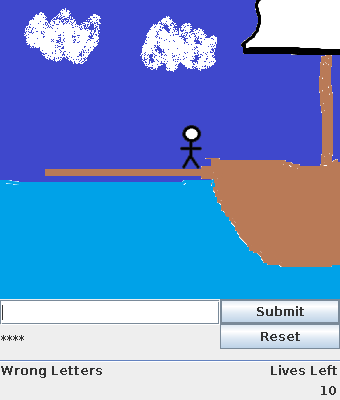
\includegraphics[scale=0.5]{TestScreenshots/0}
\caption{Screenshot 0}
\end{figure}

\begin{figure}[H]
\centering
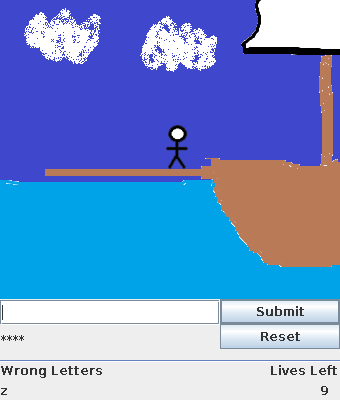
\includegraphics[scale=0.5]{TestScreenshots/1a}
\caption{Screenshot 1a}
\end{figure}

\begin{figure}[H]
\centering
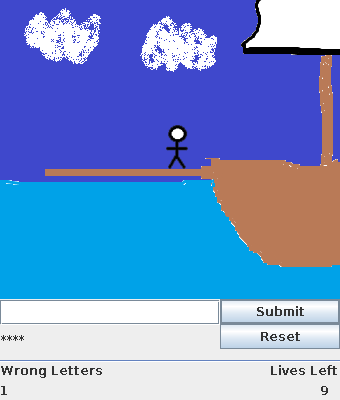
\includegraphics[scale=0.5]{TestScreenshots/1b}
\caption{Screenshot 1b}
\end{figure}

\begin{figure}[H]
\centering
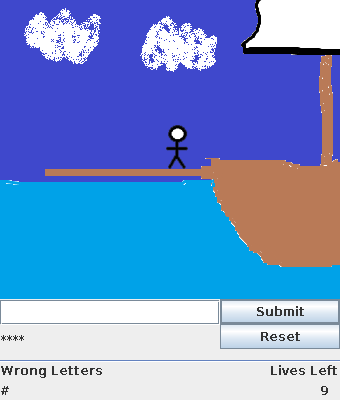
\includegraphics[scale=0.5]{TestScreenshots/1c}
\caption{Screenshot 1c}
\end{figure}

\begin{figure}[H]
\centering
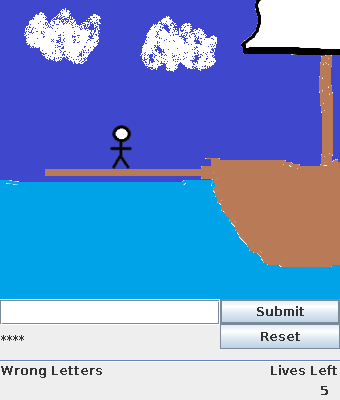
\includegraphics[scale=0.5]{TestScreenshots/1d}
\caption{Screenshot 1d}
\end{figure}

\begin{figure}[H]
\centering
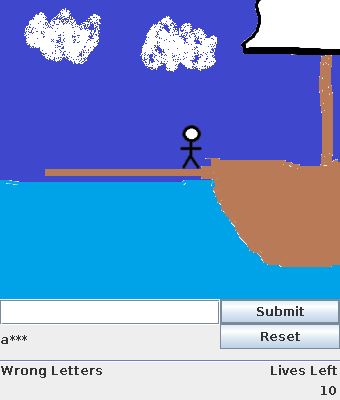
\includegraphics[scale=0.5]{TestScreenshots/2a}
\caption{Screenshot 2a}
\end{figure}

\begin{figure}[H]
\centering
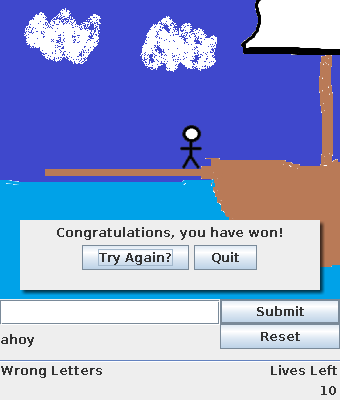
\includegraphics[scale=0.5]{TestScreenshots/2b}
\caption{Screenshot 2b}
\end{figure}

\begin{figure}[H]
\centering
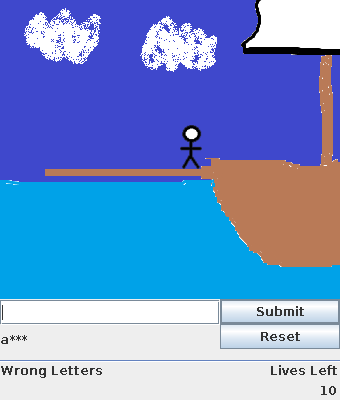
\includegraphics[scale=0.5]{TestScreenshots/3a}
\caption{Screenshot 3a}
\end{figure}

\begin{figure}[H]
\centering
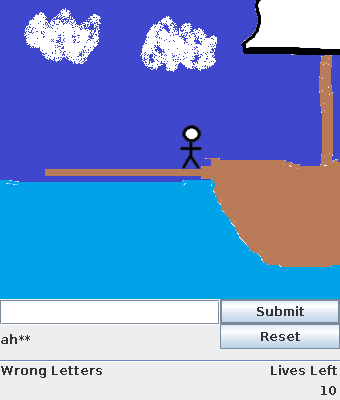
\includegraphics[scale=0.5]{TestScreenshots/3b}
\caption{Screenshot 3b}
\end{figure}

\begin{figure}[H]
\centering
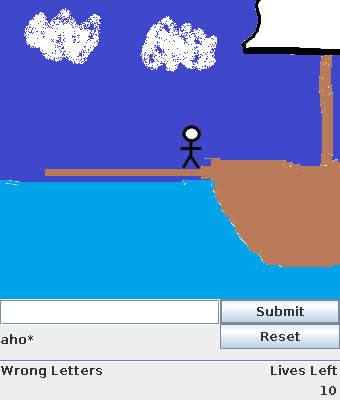
\includegraphics[scale=0.5]{TestScreenshots/3c}
\caption{Screenshot 3c}
\end{figure}

\begin{figure}[H]
\centering
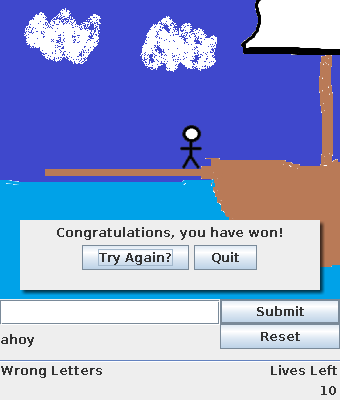
\includegraphics[scale=0.5]{TestScreenshots/3d}
\caption{Screenshot 3d}
\end{figure}

\begin{figure}[H]
\centering
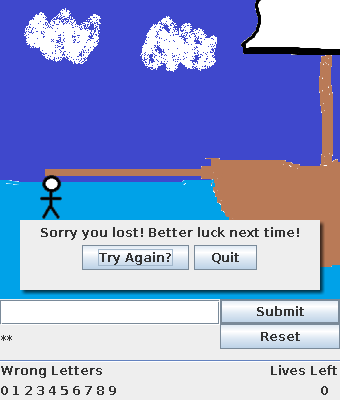
\includegraphics[scale=0.5]{TestScreenshots/4}
\caption{Screenshot 4} 
\end{figure}

\begin{figure}[H]
\centering
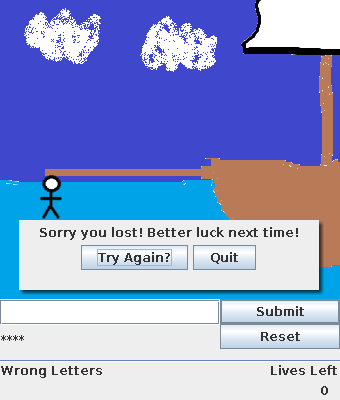
\includegraphics[scale=0.5]{TestScreenshots/5}
\caption{Screenshot 5} 
\end{figure}

\begin{figure}[H]
\centering
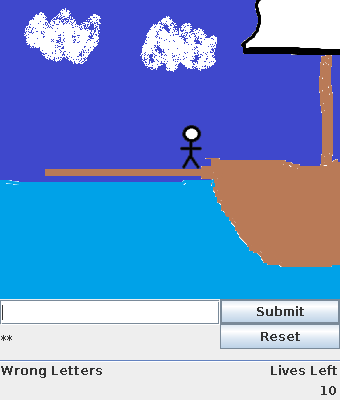
\includegraphics[scale=0.5]{TestScreenshots/6}
\caption{Screenshot 6} 
\end{figure}
\end{multicols}

\begin{figure}[H]
\centering
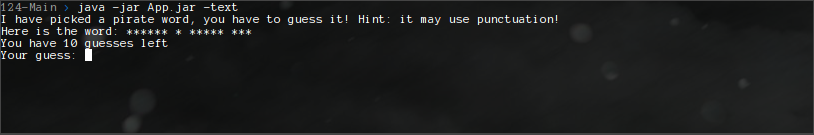
\includegraphics[scale=0.5]{TestScreenshots/7}
\caption{Screenshot 7} 
\end{figure}


\section{JUnit tests}
To make sure that my program was working to the interface that I was provided, I created some JUnit unit tests, that allowed me to quickly and easily see if the GameModel was working correctly. This was really useful and not that hard to do so it was definitely worth while. I wrote a JUnit test for each of the methods specified in the GameModelInterface. You can view the source code to see more about how I produced these tests.

Below you can see the screenshot of the results of these tests.

\begin{figure}
  \centerline{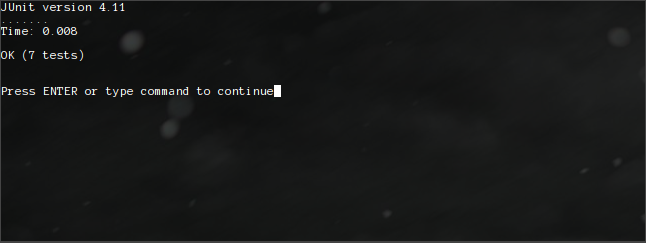
\includegraphics[scale=0.5]{junit}}
  \label{fig:label}
\end{figure}

\section{Evaluation}
Overall I think that I have done quite well on this project, my time was managed fairly well and I have created an application that meets all of the design requirements.

\subsection{Flair}
In making this project I got to learn about a few new technologies. For example I had never used Callable in Java to pass a method to another method. I used this to create the AddButton method that makes life much easier for creating eventlisteners and placing buttons on the GUI. Another technology that I am currently using is LaTeX to write this report; after using Vim to create my project it feels much more natural to be editing text in Vim and compiling it with LaTeX than it does in a traditional word processor.

As I just mentioned I didn't use an IDE for the bulk of the Java development, although in the later stages I did make an eclipse project so that I could easily generate the sequence diagram and class diagrams. I also made use of Git and had my own github repository which allowed me to use source version control making my life a lot easier!

The main bit of obvious flair to the user though is the reset button, this wasn't asked for in the specification, but I thought that it was a worthy addition to the final program as it allowed me to easily test the game, and the user to easily repeat the game. Its addition wasn't too hard but it did require a few extra methods here and there. 


\subsection{Self Evaluation}
I think that I should get at least 70\% for this assignment, as it meets all of the required specifications and is well documented and designed. That combined with the implementation of the AddButton method and the ResetButton should hopefully get me a first. 

Sadly I do feel that I may loose marks on my visuals, as the MS Paint pirate and ship are not aesthetically pleasing, and not animated. The pirate does "walk" the plank, but I think that a smoother and more intricate animation would probably have been preferred. Sadly I was unable to do this as I wanted to spend more time working on the core of the program, rather than the superficial effects.

Doing this assignment has helped me learn about working with Swing and JUnit, two things that I had never attempted before now, I was surprised by how simple and dare I say old fashioned Swing is, and once I had figured out how to actually run JUnit tests impressed by how effective and easy they were to use. I've also learned how to use LaTeX to compile this report, which I think is an invaluable skill that I had wished I had learned sooner.


\end{document}
